%-----
% Define o uso do modelo colorido ou preto e branco (escolha uma e descomente)
% Mais abaixo, defina a figura de acordo com a escolha feita.
%-----
\let \ipdf \relax

\documentclass{dct-class_bw}
%\documentclass{dct-class}

\usepackage{plain}
%\usepackage{clrscode}
%\usepackage[portugues]{algorithm2e}
%\usepackage[latin1]{inputenc}
\usepackage[utf8]{inputenc}
\usepackage{hyphenat}
\usepackage{subfig}
\usepackage{graphicx}
\usepackage{hyperref}
\graphicspath{{img/}}
\setlength{\textwidth}{16cm}

%\usepackage[portugues,ruled,vlined]{algorithm2e}
\usepackage[T1]{fontenc}
\usepackage[brazil]{babel}



\begin{document}
\thispagestyle{empty}
%----- As informações abaixo são obrigatórias  ----------------------
\titulo{ANT: Evitando Ajustes Não-essenciais em Aprendizado Incremental de Classes Agnóstico à Tarefa \\[0.3cm]
\large (ANT: Avoid Non-essential Tuning in Task-Agnostic Class-Incremental Learning)}


\autor{Tiago Clarintino Santi}
\doctipo{Monografia de Qualificação}
% Observe que a macro doctipo acima tem 2 parâmetros
% O primeiro refere-se ao nome do documento
% O segundo é sua identificação numérica, quando ela existir.
% Use a sintaxe \doctipo{XXXXX}{} quando não for
% necessária a identificação numérica--------------------------------
%--------------------------------------------------------------------
%--------------------------------------------------------------------
%----- As informações abaixo são opcionais  -------------------------

\orientacao{Edson Takashi Matsubara} \hspace{3,5cm}
%\docarea{Inteligência Artificial}

%\textofree{Monografia apresentada como requisito da qualificação
%para a obtenção do título de mestre em Ciência da Computação.}
%-----
% Se você usa o latex para compilar, comente as figuras do pdflatex
% Defina a figura do grafo a ser utilizada (escolha uma e descomente)
% Faça essa escolha de acordo com a classe escolhida (dct-class_bw ou
% dct-class)
%-----
%\vfill \centerline{\includegraphics[scale=0.8]{logo_dct_bw.mps}}
%\vfill \centerline{\includegraphics[scale=0.8]{logo_dct_color.mps}}
%-----
% Se você usa o pdflatex para compilar, comente as figuras do latex
% Defina a figura do grafo a ser utilizada (escolha uma e descomente)
% Faça essa escolha de acordo com a classe escolhida (dct-class_bw ou
% dct-class)
%-----
%\vfill\centerline{\includegraphics[scale=0.8]{logo_dct_bw-pdflatex.mps}}
%\vfill \centerline{\includegraphics[scale=0.8]{logo_dct_color-pdflatex.mps}}
\vfill \centerline{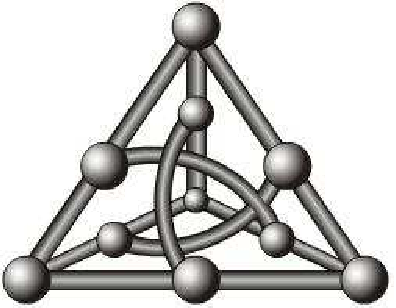
\includegraphics[scale=0.7]{grafo}}


%--------------------------------------------------------------------
% O trecho seguinte não pode ser mudado ou retirado -----------------
\vskip 0.5cm
\begin{center}
        Faculdade de Computação\\
%        Centro de Ciências Exatas e Tecnologia\\
        Universidade Federal de Mato Grosso do Sul\\
        \today
\end{center}
\newpage
\pagenumbering{roman}
%\include{resumo}
%\chapter*{Abstract}
\label{abstract}

% Redigir após a consolidação do texto principal. O conteúdo anterior a esta
% reestruturação pertencia a outro projeto e foi removido.

\textbf{Keywords}: \emph{class-incremental learning; continual learning;
task-agnostic learning; contrastive learning}.

%--------------------------------------------------------------------
% Aqui começa a inclusão dos seus textos
%
\renewcommand{\contentsname}{Sumário}
\tableofcontents

%---- O comando abaixo deve ser usado caso queira incluir o conteúdo
%como bookmark, visando facilitar a navegação no Acrobat Reader
%---------------------------------------------------------------------
%\addcontentsline{toc}{chapter}{Conteúdo}\label{conteudo}
%---------------------------------------------------------------------
%------ Aqui devem ser incluídos os capítulos ------------------------

\pagenumbering{arabic}

\chapter{Introdução}
\label{ch:introducao}

% Meta editorial: 6--9 páginas. Este capítulo deve terminar com uma cadeia
% inequívoca entre problema, pergunta, hipótese, objetivo e validação.

\section{Contextualização}
% Introduzir progressivamente aprendizado contínuo, fluxos não estacionários,
% Class-Incremental Learning (CIL), cenário agnóstico à tarefa, esquecimento
% catastrófico e dilema estabilidade--plasticidade. Delimitar o trabalho à
% classificação de imagens. Não antecipar a formulação da ANT nesta seção.

\section{Motivação e justificativa}
% Partir das limitações práticas de CIL e da interferência durante atualizações
% incrementais. Apresentar o papel dos objetivos contrastivos e a possibilidade
% de continuarem exercendo pressão sobre relações já suficientemente
% preservadas. Preparar o conceito de ajustes não essenciais sem tratá-lo como
% causa de esquecimento já comprovada.

\section{Problema de pesquisa}
% Formular independentemente da solução: em métodos incrementais com
% destilação contrastiva, relações já suficientemente preservadas podem
% continuar contribuindo para o gradiente, produzindo atualizações
% potencialmente desnecessárias e interferência adicional ao aprender novas
% classes. Definir depois, no Capítulo 3, o que "suficientemente preservada" e
% "não essencial" significam operacionalmente.

\section{Questões de pesquisa}

\subsection{Questão principal}
% Investigar se restringir atualizações contrastivas às relações que ainda
% violam um critério de preservação reduz interferência sem prejudicar o
% aprendizado de novas classes e o desempenho incremental.

\subsection{Questões secundárias}
% Manter apenas questões respondidas pelos experimentos:
% (Q1) referência compartilhada ou por âncora na ANT;
% (Q2) cobertura intra-view ou simétrica completa;
% (Q3) normalização nGlobal/nLocal e sua equivalência efetiva;
% (Q4) comportamento das métricas internas do mecanismo;
% (Q5) efeito sobre accuracy e forgetting entre datasets e sementes.

\section{Hipóteses de pesquisa}

\subsection{Hipótese principal}
% H1: restringir a otimização contrastiva às violações relevantes reduz
% atualizações não essenciais sem comprometer a aquisição de novas classes,
% preservando ou melhorando o desempenho incremental. Formular também H0.

\subsection{Hipóteses auxiliares e critérios de interpretação}
% Criar uma hipótese auxiliar somente para decisões com comparação controlada.
% Para cada hipótese, registrar: métrica -> experimento -> evidência esperada ->
% critério para suportada, não suportada ou inconclusiva. Não considerar uma
% diferença pequena de uma única semente como confirmação isolada.

\section{Objetivos}

\subsection{Objetivo geral}
% Desenvolver e avaliar um método para evitar atualizações contrastivas não
% essenciais em CIL agnóstico à tarefa, tendo a ANT como proposta central.

\subsection{Objetivos específicos}
% Caracterizar o problema; formular a ANT; investigar referência e cobertura;
% auditar nGlobal/nLocal; desenvolver diagnósticos do mecanismo; avaliar em
% diferentes datasets/protocolos/sementes; comparar com TagFex e baselines
% adequados. Avg-K e SBS não são objetivos centrais.

\section{Escopo e delimitações}
% Fixar protocolo, informação disponível no treino/teste, memória limitada,
% backbones, datasets e métricas. Distinguir task-agnostic na inferência de
% task-free/boundary-free no treinamento. Separar trabalho consolidado de
% extensões ainda exploratórias.

\section{Contribuições esperadas}
% Hierarquia obrigatória:
% (1) contribuição principal: ANT;
% (2) decisões metodológicas: aGlobal/aLocal, intra-view/aSymFull e auditoria
%     nGlobal/nLocal;
% (3) formulações alternativas como ablações;
% (4) investigações auxiliares: Avg-K e SBS;
% (5) extensões: colisões entre tarefas e negativos baseados em protótipos.

\section{Organização do trabalho}
% Cap. 2: fundamentos, TagFex e lacuna; Cap. 3: ANT, decisões, validação e
% evidências preliminares; Cap. 4: trabalho restante até a defesa.

\chapter{Fundamentação Teórica e Trabalhos Relacionados}
\label{ch:fundamentacao}

% Meta editorial: 12--17 páginas. Narrativa: CIL -> interferência -> famílias
% de métodos -> contraste -> destilação contrastiva -> TagFex -> ponto de
% intervenção -> literatura relacionada -> lacuna.

\section{Aprendizado contínuo e incremental de classes}

\subsection{Definição e notação do cenário incremental}
% Definir amostras, rótulos, etapas, classes disjuntas, memória de exemplares,
% espaço de saída acumulado e avaliação após cada etapa.

\subsection{Protocolos e informação de tarefa}
% Diferenciar Task-IL, Domain-IL e Class-IL; task-aware, task-agnostic na
% inferência e task-free/boundary-free no treinamento. Declarar o protocolo
% efetivamente usado pelo TagFex e por este trabalho.

\section{Esquecimento, interferência e estratégias de mitigação}

\subsection{Estabilidade, plasticidade e fontes de erro}
% Relacionar esquecimento, interferência, deriva de representação, viés do
% classificador e desbalanceamento. Não atribuir toda queda a um único mecanismo.

\subsection{Repetição, regularização e expansão arquitetural}
% Revisão focada de rehearsal/herding, destilação, expansão dinâmica e métodos
% híbridos; explicitar custos e pressupostos.

\subsection{Alinhamento e classificação por médias de classe}
% Preparar weight alignment, protótipos e NME usados no pipeline de referência.

\section{Aprendizado contrastivo e destilação contrastiva}

\subsection{Embeddings, similaridade e pares contrastivos}
% Normalização L2, cosseno, temperatura, duas views, âncora, positivo, negativos
% e estrutura da matriz 2B x 2B.

\subsection{InfoNCE e fluxo de gradientes}
% Derivar a perda por âncora e interpretar cada termo. Explicar o que continua
% contribuindo para o gradiente, sem concluir antecipadamente que todo gradiente
% residual seja prejudicial.

\subsection{Destilação contrastiva em aprendizado incremental}
% Distinguir contraste aluno--aluno de destilação aluno--professor e explicar
% por que esse segundo caso é o foco científico do problema.

\subsection{Ponte para os ajustes não essenciais}
% Revisar a motivação da literatura e formular a possibilidade de relações já
% preservadas continuarem ativas. A definição e solução pertencem ao Cap. 3.

\section{TagFex como método de referência}

\subsection{Arquitetura e visão geral do pipeline}
% Expansão de atributos específicos à tarefa, ramo agnóstico, projetor,
% preditor e cabeças. Inserir figura: TagFex -> destilação contrastiva -> ponto
% exato em que a ANT intervém.

\subsection{Primeira etapa e etapas incrementais}
% Explicar expansão, congelamento, professor, duas views, replay e diferenças
% entre o primeiro treinamento e os seguintes.

\subsection{Termos da função objetivo}
% Reunir classificação principal, cabeça/perda auxiliar, contraste,
% destilação contrastiva, classificação de transferência e KL condicional.
% Interpretar coeficientes e o fator automático de destilação.

\subsection{Memória, herding, NME e alinhamento de pesos}
% Explicar quando cada operação ocorre e como participa da avaliação.

\subsection{Uma etapa incremental passo a passo}
% Pseudocódigo/fluxograma alinhado a train() e _compute_incremental_loss() de
% tagfex_clean.py. Encerrar identificando a chamada contrastiva modificada.

\section{Ponto de intervenção e lacuna científica}
% Mostrar em que termo do TagFex as relações contrastivas são construídas, por
% que o critério de ativação é relevante e o que o método-base não controla.
% Não apresentar ainda todas as decisões aGlobal/aLocal/aSymFull.

\section{Trabalhos relacionados}

\subsection{Métodos de CIL diretamente comparáveis}
% TagFex, DER, iCaRL e apenas baselines efetivamente comparáveis.

\subsection{Seleção contrastiva, margens e preservação de representações}
% Revisão curta das linhas mais próximas ao mecanismo proposto.

\subsection{Síntese e transição para a proposta}
% Responder: o que existe, o que cobre, o que falta e como essa lacuna motiva a
% ANT. Terminar apontando diretamente ao Capítulo~\ref{ch:proposta}.

\chapter{Proposta Metodológica}
\label{ch:proposta}

% Meta editorial: 22--32 páginas. Este é o capítulo central. A ordem narrativa
% é problema -> formulação -> decisões de projeto -> diagnósticos -> validação.

\section{Visão geral da ANT}
% Responder antes das equações: qual problema resolve; que similaridades usa;
% quais relações deixam de produzir pressão; quais continuam ativas; onde a
% ANT entra na destilação contrastiva do TagFex. Inserir diagrama comparando
% TagFex e TagFex+ANT.

\section{Atualizações contrastivas não essenciais}

\subsection{Cenário motivador e interpretação geométrica}
% Exemplo visual pequeno com âncora, positivo, negativos adequados e violadores.
% Mostrar intuitivamente por que relações adequadas não precisam receber a
% mesma pressão de otimização indefinidamente.

\subsection{Definição operacional e consequências esperadas}
% Distinguir loss residual, gradiente não nulo, violação de margem, atualização
% não essencial e dano ao conhecimento anterior. Definir quais serão observáveis
% e quais permanecem inferências a testar.

\subsection{Predições e diagnósticos do mecanismo}
% Se a hipótese estiver correta: adjusted loss, active ratio, distribuição de
% violações e hard-negative similarity devem evoluir de forma compatível, sem
% perda de plasticidade medida no desempenho das novas classes.

\section{Formulação base da ANT}
% Desenvolver em sequência, com interpretação após cada equação:
% (1) batch e duas views; (2) embeddings normalizados; (3) matriz de
% similaridade; (4) máscaras de self/positivos; (5) negativos válidos;
% (6) referência; (7) margem; (8) v_ij = s_ij - r + gamma;
% (9) termos ativos; (10) agregação; (11) L_ANT;
% (12) alpha L_InfoNCE + beta L_ANT; (13) fluxo de gradientes.
% Conferir tudo contra _build_ant_matrix(), _compute_ant_loss() e
% _compute_contrastive_loss_base() antes da redação definitiva.

\section{Decisão de projeto I: referência da ANT}

\subsection{Referência global (aGlobal)}
% Um valor compartilhado extraído do domínio válido da matriz ANT. Formalizar
% domínio, acoplamento entre âncoras, margem efetiva e gradientes esperados.

\subsection{Referência por âncora (aLocal)}
% Máximo por linha. Formalizar a diferença para aGlobal e discutir adaptação a
% graus distintos de dificuldade, sem declarar benefício antes das ablações.

% Inserir tabela: variante | domínio da referência | granularidade | efeito
% esperado | hipótese/experimento.

\section{Decisão de projeto II: cobertura da matriz}

\subsection{Cobertura intra-view assimétrica}
% Variante original: bloco Q1/S11, B âncoras e B-1 negativos. Explicitar quais
% views e blocos não participam.

\subsection{Cobertura simétrica completa (aSymFull)}
% Matriz 2B x 2B, removendo self e par positivo; 2B-2 negativos por âncora.
% Explicar simetria, cobertura, custo e comportamento esperado.

% Figura obrigatória: Q1, Q2, Q3, Q4, self, positivos, negativos e blocos usados
% por cada variante. Tabela: referência | cobertura | granularidade | custo.

\section{Decisão associada: normalização da InfoNCE}

\subsection{Normalização nGlobal e nLocal}
% Apresentar as duas formas lado a lado, por linha, com matriz pequena. Tratar
% como decisão da InfoNCE, separada da referência ANT.

\subsection{Equivalência algébrica e verificação numérica}
% A implementação nLocal subtrai uma constante por linha antes de uma expressão
% invariável a deslocamentos. Demonstrar condições de equivalência, comparar
% valores/gradientes e só então discutir estabilidade de ponto flutuante.
% TODO crítico: resolver a inconsistência entre a narrativa histórica de
% gradientes balanceados e a implementação atual.

\subsection{Combinações das decisões}
% aGlobal+nGlobal, aGlobal+nLocal, aLocal+nGlobal, aLocal+nLocal e aSymFull com
% a normalização correspondente. Explicar que são produtos de decisões
% independentes, não cinco métodos autônomos.

\section{Formulações alternativas como ablações}
% Consolidar logsumexp, expm1, softplus, top-k e active-only em uma tabela:
% motivação | diferença matemática | comportamento esperado | hipótese |
% experimento/status. Não elevar alternativas sem evidência a contribuições.
% Explicar aqui o piso log(N_valid) da logsumexp e a diferença entre problema
% diagnóstico e problema de otimização.

\section{Investigações auxiliares}

\subsection{Avg-K: estabilização temporal do professor}
% Média dos últimos K checkpoints de ta_net/projector; relação complementar ou
% independente da ANT; K=3/5/10; custo e evidência disponível. Não apresentar
% como contribuição principal sem suporte adicional.

\subsection{SBS: seleção de exemplares por velocidade de aprendizagem}
% Score por acertos/tentativas, filtragem das caudas, herding posterior,
% relação com rehearsal e limitações atuais (FFCV/distribuído).

\section{Algoritmo integrado}

\subsection{TagFex baseline e TagFex+ANT}
% Pseudocódigo comparável: forward -> professor -> matriz -> InfoNCE ->
% referência/margem/máscara ANT -> combinação -> backward -> atualização ->
% memória -> alinhamento -> avaliação. Destacar visualmente as linhas novas.

\subsection{Integração opcional dos mecanismos auxiliares}
% Mostrar Avg-K/SBS como módulos opcionais após o núcleo, não como parte
% necessária da definição da ANT. Incluir complexidade de tempo/memória.

\section{Metodologia experimental}

\subsection{Matriz de hipóteses e experimentos}
% Tabela obrigatória: pergunta/hipótese | comparação controlada | datasets |
% seeds/status | métricas de desempenho | métricas de mecanismo.

\subsection{Protocolos e reprodutibilidade}
% Datasets e divisões; classes iniciais/incrementais; seeds; arquitetura;
% épocas; batch e views; memória; hiperparâmetros; baselines; hardware;
% configuração e origem do resultado. Marcar completo/parcial/em execução/falha.

\subsection{Métricas e análise estatística}
% Avg Acc@1, NME@1, desempenho final, forgetting e curvas; raw/adjusted loss,
% active ratio, hard-negative similarity, violações/percentis e gaps; média,
% dispersão, tamanho de efeito e testes compatíveis com o desenho final.

\section{Resultados preliminares e análise do mecanismo}

\subsection{Comportamento interno da ANT}
% Estrutura de cada resultado: hipótese -> expectativa -> métrica -> figura ->
% observação -> interpretação -> limitação. Explicar matematicamente o piso:
% log(254) ~= 5,54; raw loss quase plana não implica ausência de aprendizado.
% Analisar adjusted loss, active ratio, hard negatives e percentis.

\subsection{Desempenho incremental e ablações}
% Accuracy/NME/forgetting com múltiplas seeds quando disponíveis; separar
% resultados completos, parciais, em execução, falhos e exploratórios.
% Organizar por decisão: referência, cobertura, normalização, formulação;
% Avg-K/SBS vêm depois como investigações auxiliares.

\subsection{Síntese das hipóteses}
% Classificar evidência como forte, tendência, inconclusiva ou não sustentada.
% Não converter diferenças pequenas de uma seed em superioridade.

\section{Ameaças à validade e limitações}
% Em uma seção coesa: validade interna, externa e de construto; seeds;
% hiperparâmetros; baseline; datasets/backbones; custo; dependência do TagFex;
% relação entre proxies geométricas e atualização realmente não essencial.

\section{Extensões em investigação}
% Separar da contribuição defendida: colisões entre tarefas, negativos baseados
% em protótipos antigos e outras estratégias somente após validação diagnóstica.

\chapter{Plano de Trabalho e Cronograma}
\label{ch:plano-trabalho}

% Meta editorial: 3--5 páginas. Capítulo curto, verificável e prospectivo.

\section{Estado atual}
% Tabela/inventário datado: escrita, implementação, experimentos concluídos,
% em execução, incompletos, falhos e análises disponíveis. Não inferir status
% apenas pela existência de configs; confirmar logs/reports.

\section{Trabalho restante até a defesa}
% Organizar por entregável: auditoria texto-código (inclusive nLocal/nGlobal),
% experimentos principais restantes, análise estatística, figuras, redação,
% revisão com orientação e preparação da defesa. Avg-K/SBS e extensões não podem
% bloquear o núcleo mínimo de validação da ANT sem justificativa explícita.

\section{Cronograma mensal e marcos}
% Tabela mês x atividade, com legenda planejado/em andamento/concluído e marcos
% observáveis. TODO: preencher datas somente após confirmar calendário do
% programa e alinhar o conjunto mínimo de experimentos com a orientação.

\section{Riscos e contingências}
% GPU/tempo, variância, experimentos incompletos, equivalência nLocal/nGlobal,
% resultados inconclusivos e redução de escopo. Definir plano mínimo para
% responder à hipótese principal mesmo que investigações auxiliares falhem.

\section{Critérios de conclusão}
% Condições para encerrar experimentação, análise, redação, revisão e defesa.


%---------------------------------------------------------------------
% Aqui está um exemplo de bibliografia
% Veja o arquivo bibi_exemplo.bib
% Para você ter um " GUIA "
%---------------------------------------------------------------------
%%\refstepcounter{chapter}
%%\refstepcounter{chapter}% Adiciona 1 to chapter ou seja (\thechapter=\thechapter+1)
%%\addcontentsline{toc}{chapter}{Referências
%%Bibliográficas}\label{bibliografia} \nocite{*}

%-----
% Define o estilo das referências bibliográficas
%-----
%\bibliographystyle{dct-alpha}
\bibliographystyle{dct-plain}
%\nocite{*}
\bibliography{referencias}
%--------------------------------------------------------------------
\end{document}
